%==============================================================================
\section{Trabalhos Relacionados}\label{sec:trabalhosRelacionados}
%==============================================================================
Para investigar os trabalhos relacionados a esta pesquisa foi utilizado um mapeamento sistemático da literatura. Ele consiste em três etapas, a definição do protocolo do mapeamento, a execução do protocolo e a análise dos resultados.


%------------------------------------------------------------------------------
\subsection{Protocolo do mapeamento}\label{sub:trabalhosRelacionados_metodologia}
%------------------------------------------------------------------------------
O objetivo do protocolo é estabelecer o estado da arte das ferramentas que dão apoio a execução de processos baseados em SPEM. Baseado nisso, foi definido apenas uma questão de pesquisa para investigar nos trabalhos selecionados, sendo ela: Quais as funções e objetivos das ferramentas?

O mecanismo de busca escolhido foi o Google Scholar \footnote{Google Scholar \url{http://scholar.google.com}}, levando em consideração que ele indexa a maior parte das bases de dados. A \textit{string} de busca utilizada foi ``software process''+``tool'' OR ``tools'' OR ``CASE'' + ``software \& systems process engineering metamodel'' OR ``SPEM''. Para filtrar a busca, definimos os seguintes critérios de inclusão.

\begin{itemize}
	\item Artigos completos publicados de 2012 até 2017 e com no mínimo 6 (seis) páginas;
	\item Artigos que abordam sobre ferramentas de suporte ao SPEM.
\end{itemize}

Para retirar trabalhos que não são interessantes para esta pesquisa definimos dois critérios de exclusão.
\begin{itemize}
	\item Artigos que sejam outros mapeamentos ou revisões sistemáticas;
	\item Artigos repetidos ou versões resumidas de trabalhos completos.
\end{itemize}
De acordo com os trabalhos retornados, o modo de classificação definido foi pelo ano e o veículo de publicação.

%------------------------------------------------------------------------------
\subsection{Resultado}\label{sub:trabalhosRelacionados_resultados}
%------------------------------------------------------------------------------
A execução do protocolo retornou 2060 trabalhos, com a aplicação dos critérios de inclusão este número reduziu para 726 e após aplicar os critérios de exclusão 19 trabalhos foram selecionados para leitura e análise mais aprofundada. Dentre os trabalhos, nenhum apresentou ferramentas para apoiar a execução de processos, servindo de suporte para guiar e gerenciar as etapas do processo em sua execução.

%Para dar um panorama geral dos trabalhos que encontrados, são exibidos de acordo com sua classificação, pelos anos de publicação e seus veículos de pesquisa.

\subsubsection{Classificação dos resultados}
Para visualizar a quantidade de publicações pelos anos, é exibido na Figura \ref{fig:graf} os trabalhos selecionados de acordo com seu ano de publicação. A grande maioria está entre os anos de 2012 a 2014, sendo a concentração maior no ano de 2012, seguido de 2013 e 2014. Os anos de 2015 e 2016 são equivalentes em relação a quantidade de publicações. Desta forma, nos últimos anos as publicações sobre este assunto apresentam uma queda de quantidade. Isso é visível apenas observando a Figura \ref{fig:graf}, sendo que não existem trabalhos selecionados do ano de 2017.
\begin{figure}[!htb]
	\caption{Gráfico do ano das publicações e dos veículos}\label{fig:graf}
	\begin{center}
		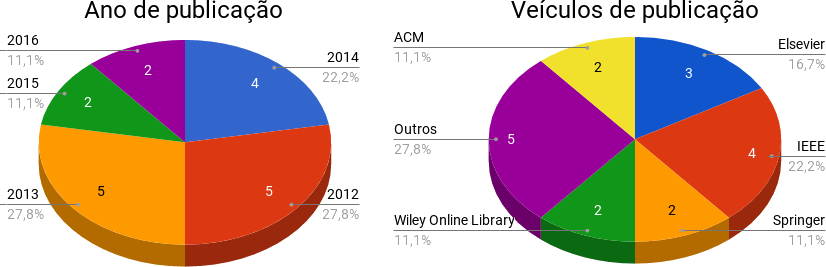
\includegraphics[scale=0.5]{img/graf}
	\end{center}
	%\legend{}
\end{figure}

Com a intenção de identificar onde ocorrem a maior parte das publicações dos trabalhos selecionados, eles foram classificados de acordo com seu veículo de publicação, exibidos na Figura \ref{fig:graf}. A maior quantidade está na fatia chamada outros, que engloba trabalhos de bases de universidades e de veículos de menor expressão. Esse agrupamento foi realizado para melhorar a exibição dos dados. Dentre os veículos mais conhecidos a IEEE lidera com 4 trabalhos (ou 21,1\%) seguida pela Elsevier com 3 trabalhos (ou 15,8\%).

%\begin{figure}[!htb]
%	\caption{Gráfico do veículos das publicações}\label{fig:veiculo}
%	\begin{center}
%		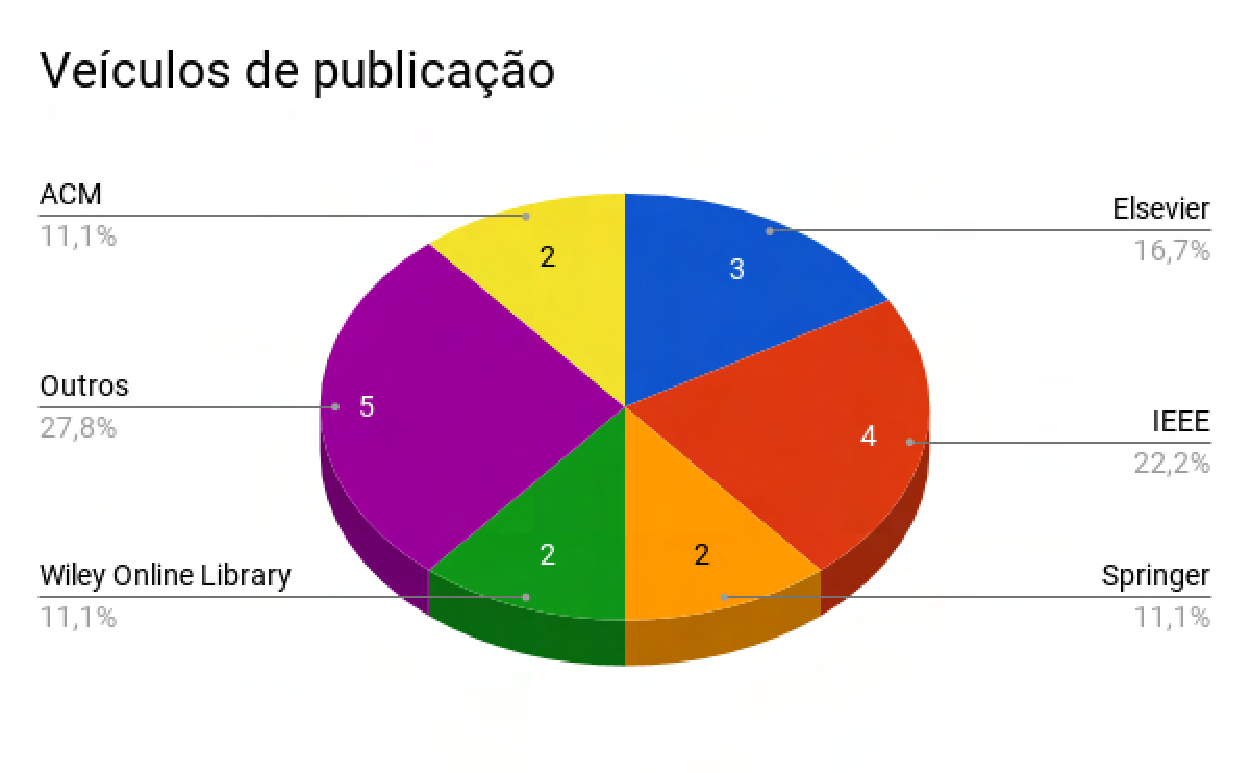
\includegraphics[scale=0.4]{img/GrafVeiculo}
%	\end{center}
	%\legend{}
%\end{figure}

Após uma exibição geral dos trabalhos, a seguir são exibidas as respostas dos trabalhos para a questão de pesquisa definida no protocolo.
%------------------------------------------------------------------------------
\subsubsection{Qual a função e objetivo das ferramentas?}\label{subsub:trabalhosRelacionados_resultados_questao1}
%------------------------------------------------------------------------------

 Kuhrmann et al. (2043) apresentam a ferramenta Process Enactment Tool Framework (PET), que tem como objetivo transformar determinados modelos de processo formal em um formato que as ferramentas de projetos de processos possam interpretar, ou seja,  O PET é um instrumento para importar processos com base em um metamodelo e fornecer exportações para um ambiente de projeto específico \cite{1kuhrmann:2014}. Ellner et al. (2012) apresentam uma cadeia de ferramentas integrada baseada em eSPEM e Eclipse. Elas suportam modelos de processo baseados em eSPEM e também orienta e apoia a equipe de projeto a trabalhar de acordo com o processo de maneira sensível ao contexto. Elas automatizam o trabalho repetitivo e pesado como verificação de conformidade do processo ou acompanhamento de progresso \cite{10ellner:2012}. Já Hurtado et al.(2013) propõem uma abordagem orientada por modelo para especificação e configuração de linhas de processo de software \cite{8hurtado:2013}. Entrando nas metodologias ágeis Abad, Alipour e Ramsin (2012)  propõem um \textit{plug-in} para o EPFC, para permitir aos engenheiros de métodos construir metodologias ágeis através de uma abordagem de PME baseada em montagem. O \textit{plug-in} fornece facilidades para a especificação das características de um determinado projeto, seleção de componentes de processo ágeis adequados do repositório de métodos e montagem final dos pedaços de método selecionados \cite{13abad:2012}.
 
 
Três trabalhos abordam sobre implantação de melhorias e avaliação em processos de softwares, como Portela et al. (2014) apresentam um conjunto de ferramentas de suporte para a implementação de processos modelados no SPEM. Este conjunto de ferramentas, é chamada Spider-PE e tem como objetivo auxiliar as organizações de software na implementação do Modelo de Maturidade de Capacidades para Desenvolvimento (CMMI-DEV) e do Modelo de Referência de Melhoria de Processos de Software para Software (MR-MPS- SW) \cite{9portela:2014}. Hurtado, Bastarrica e Bergel (2013) apresentam uma ferramenta que permite analisar a qualidade dos modelos de processos de software SPEM 2.0. A ferramenta chamada Avispa, identifica uma série de padrões de erro e os destaca em planos diferentes. Uma descrição detalhada dos internos da Avispa é fornecida para mostrar sua estrutura e seus mecanismos de extensibilidade. Além disso, os autores apresentam um mecanismo interativo para definir novos \textit{scripts} de análise e implementar novos padrões e planos \cite{6hurtado:2013}. 
Já se tratando de avaliação, Gazel, Sezer e Tarhan (2012) apresentam uma ferramenta de avaliação de processo de software baseada em ontologia para coleta de dados da avaliação de processos e acompanhar a conformidade dos processos de software com o CMMI como modelo de referência do processo \cite{7gazel:2012}. 



%Adaptação de Processos
Muitos trabalhos selecionados abordam sobre adaptação de processos, definindo algumas variáveis para adaptar da melhor maneira o processo para determinado escopo, dentre esses trabalhos, Silvestre, Bastarrica e Ochoa 2014, apresentam uma ferramenta baseada em modelo que permite aos engenheiros de processos gerar automaticamente regras de transformação de adaptação usando uma interface gráfica de usuário \cite{3silvestre:2014}. Hurtado et al (2013) mostram uma abordagem baseada em modelo para a adaptação de processos de software, gerando automaticamente processos específicos do projeto com base no processo organizacional e nos contextos do projeto \cite{11hurtado:2013}. Casare et al (2016) expõem Medusa, uma abordagem para adaptar processos de desenvolvimento de acordo com as necessidades do projeto. Ela se baseia em técnicas e métodos de engenharia de linha de produtos, leva em consideração as semelhanças e diferenças do processo, bem como fragmentos reutilizáveis \cite{16casare:2016}. Santos et al. (2015) relatam uma técnica que usa a mineração de processos para descobrir elementos do processo de software que são candidatos a adaptação. A abordagem analisa os \textit{logs} de execução de várias instâncias de processo que compartilham um processo padrão comum \cite{17santos:2015}. Chaghrouchni, Kabbaj e Bakkoury (2014) apresentam uma nova abordagem para a evolução do processo, com base na adaptação dinâmica. Ao identificar os desvios do processo a adaptação dinâmica é usada para decidir a nova atividade ou conjunto de atividades a serem lançadas para reproduzir entradas e saídas solicitadas e para lidar com o impacto de desvio \cite{18chaghrouchni:2014}.

%------------------------------------------------------------------------------
Vários trabalhos estão relacionados com tratamento de variabilidades, como o de Rouillé et al. (2013) que propõe uma abordagem para resolução de variabilidades de processos em Linhas de Processos de Software durante a execução do processo \cite{14rouille:2013}. Em outro trabalho Rouillé et al. (2012) relatam uma abordagem para definição de uma Linha de Processo de Software e a derivação automática de um processo a partir desta SPL de acordo com os requisitos de um determinado projeto. A variabilidade é gerenciada separadamente do modelo de processo utilizando uma linguagem de variabilidade comum \cite{2rouille:2012}. Simmonds et al. (2012) apresentam uma combinação de notações e ferramentas para formalizar modelos de processos de software incluindo sua variabilidade, utilizando a ferramenta Modisco/AMW para garantir que somente a variabilidade razoável seja especificada \cite{12simmonds:2012}. Blum, Simmonds e Bastarrica (2015) propõem o algoritmo V que usa dois processos limiares para configurar uma Linha de Processo de Software. Relações muito frequentes são usadas para construir o processo base, as relações variáveis definem a variabilidade do processo e as relações raras são descartadas como ruídos \cite{15blum:2015}. Ayora et al. (2016) derivaram um conjunto de padrões de mudança para famílias de processos de construções de linguagem específicas de variabilidade identificadas na literatura, com objetivo de facilitar o gerenciamento de variabilidade nas famílias de processos, garantindo a correção familiar do processo e reduzir o esforço necessário para tais fins \cite{19ayora:2016}.


